\documentclass[UTF8,12pt]{ctexart}
\usepackage{graphicx}
\usepackage{amsmath}
\usepackage{graphicx}
\usepackage{bm}
\usepackage{geometry}
\geometry{left=3.0cm,right=3.0cm,top=2.0cm,bottom=2.0cm}
\title{test}
\author{魏文彬}
\begin{document}
%\maketitle
\subsection*{PCA算法推导}
这里采用最小误差的形式推导,因为在推导过程中我们用到原始数据的一种近似表示,
引入$D$维基向量的完整单位正交集合$\{\bm{u}_i\}$,其中$i=1,\dots,D$,满足
\begin{equation}
	\bm{u}_i^T\bm{u}_j=\delta_{ij}
\end{equation}
每个数据点可以精确地表示为基向量的线性组合,即
\begin{equation}
    \bm{x}_n=\sum_{i=1}^n \alpha_{ni} \bm{u}_i
\end{equation}
将$\bm{x}_n$与$\bm{u}_j$做内积,利用单位正交性,可得$\alpha_{nj}=\bm{x}_n^T\bm{u}_j$,因此不失一般性,我们有
\begin{equation}
    \bm{x}_n=\sum_{i=1}^D(\bm{x}_n^T\bm{u}_i)\bm{u}_i
\end{equation}
现在我们使用$M(M<D)$维的线性子空间来近似表示$\bm{x}_n$,不失一般性,采用$D$维子空间的前$M$个基向量,即
\begin{equation}
    \tilde{\bm{x}}_n=\sum_{i=1}^M z_{ni}\bm{u}_i+\sum_{i=M+1}^D b_i\bm{u}_i
\end{equation}
其中$\{z_{ni}\}$依赖于特定的数据点,$\{b_i\}$是常数对所有的数据点都相同。我们的目标是选择$\{\bm{u}_i\}$,$\{z_{ni}\}$,$\{b_i\}$最小化失真函数
\begin{equation}
    J=\frac{1}{N}\sum_{i=1}^N \Vert \bm{x}_n-\tilde{\bm{x}}_n\Vert^2
\end{equation}
首先考虑$\{z_{nj}\}$,注意这里$J,z_{nj}$是标量,$\tilde{\bm{x}}_n$是向量
\begin{equation}
\frac{\partial J}{\partial z_{nj}} = (\frac{\partial \tilde{\bm{x}}_n}{\partial z_{nj}})^T \frac{\partial J}{\partial \tilde{\bm{x}}_n} 
= \bm{u}_j^T(2\tilde{\bm{x}}_n-2\bm{x}_n)
=2(\bm{x}_n^T \bm{u}_j-z_{nj})
\end{equation}
另上式等于0,可得
\begin{equation}
    z_{nj} = \bm{x}_n^T\bm{u}_j
\end{equation}
考虑$b_j$
\begin{equation}
\frac{\partial J}{\partial b_j} = (\frac{\partial \tilde{\bm{x}}_n}{\partial b_j})^T \frac{\partial J}{\partial \tilde{\bm{x}}_n} 
=\frac{1}{N} \sum_{j=1}^N \bm{u}_j^T(2\tilde{\bm{x}}_n-2\bm{x}_n)
=\frac{2}{N}\sum_{j=1}^N (\bm{x}_n^T \bm{u}_j-b_j)
\end{equation}
另上式为0,可得
\begin{equation}
	b_j=\bar{\bm{x}}^T\bm{u}_j
\end{equation}
其中$j=M+1,\cdots,D$,误差向量为
\begin{equation}
	\bm{x}_n-\tilde{\bm{x}}_n = \sum_{i=M+1}^D\{(\bm{x}_n-\bar{\bm{x}}^T)\bm{u}_i\}\bm{u}_i
\end{equation}
可以看到误差向量位于与主子空间垂直的空间中。
将上面的结果带入失真度量$J$,我们得到下式,它是一个纯粹关于$\{\bm{u}_i\}$的函数
\begin{equation}
	J=\frac{1}{N}\sum_{n=1}^N\sum_{i=M+1}^D(\bm{x}_n^T\bm{u}_i-\bar{\bm{x}}^T\bm{u}_i)^2
	=\sum_{i=M+1}^D\bm{u}_i^TS\bm{u}_i
\end{equation}
剩下是求$\{\bm{u}_i\}$使$J$最小化。考虑$D=2,M=1$的情况,我们限制$\bm{u}_2^T\bm{u}_2=1$,引入拉格朗日乘子$\lambda_2$,等价于最小化下式
\begin{equation}
	\tilde{J}=\bm{u}_2^TS\bm{u}_2+\lambda_2(1-\bm{u}_2^T\bm{u}_2)
\end{equation}
另上式关于$\bm{u}_2$的导数等于0,得到$S\bm{u}_2=\lambda_2\bm{u}_2$,从而$\bm{u}_2$是$S$的特征向量,特征值为$\lambda_2$。
对于任意的$D$和任意的$M<D$,最小化$J$的解可以求协方差矩阵的特征向量得到,即
\begin{equation}
	S\bm{u}_i=\lambda_i\bm{u}_i
\end{equation}
其中$i=1,\cdots,D$,这里特征向量$\{\bm{u}_i\}$是单位正交的,失真度量为
\begin{equation}
	J = \sum_{i=M+1}^D\lambda_i
\end{equation}
\subsection*{PCA应用}
PCA的一种应用是数据的降维压缩,另一种用途是数据预处理,我此次作业实现的是PCA对图片的压缩。
我们再看一下数据的近似过程,压缩就体现在这个近似过程中,将求得的结果带入(4)式中,可以得到数据的近似
\begin{equation}
\tilde{\bm{x}}_n = \sum_{i=1}^M(\bm{x}_n^T \bm{u}_i)\bm{u}_i+\sum_{i=M+1}^D(\bar{\bm{x}}^T\bm{u}_i)\bm{u}_i
	=\bar{\bm{x}}+\sum_{i=1}^M(\bm{x}_n^T\bm{u}_i-\bar{\bm{x}}^T\bm{u}_i)\bm{u}_i
\end{equation}
由上式重构出$\tilde{\bm{x}}_n$,我们需要
\begin{itemize}
	\item $\bar{\bm{x}}$,$D$维向量,数据量$D\times 1$
	\item $\{\bm{u}_i\}$,$M$个基向量,数据量$D \times M$
	\item $\bm{x}_n^T\bm{u}_i-\bar{\bm{x}}^T\bm{u}_i$,对应于基向量的$M$个系数,$N$个数据共$N \times M$个数据量。
\end{itemize}
这里我们先引入一个压缩率$R$的定义,$R$定义为重构数据需要的数据量比上原始数据数据量,即
\begin{equation}
	R=\frac{D+D\times M+M\times N}{D\times N}
\end{equation}
\subsection*{计算结果}
分别对灰度图与RGB彩色图进行了PCA,其中的压缩率用式(16)计算,结果如下
\\
\begin{figure}
	\centering
	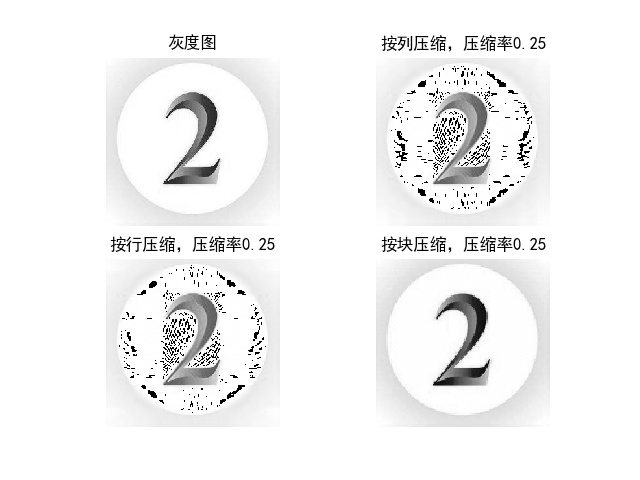
\includegraphics[width=.8\textwidth]{L.jpeg}
	\caption{灰度图PCA}
\end{figure}
\\
\begin{figure}
	\centering
	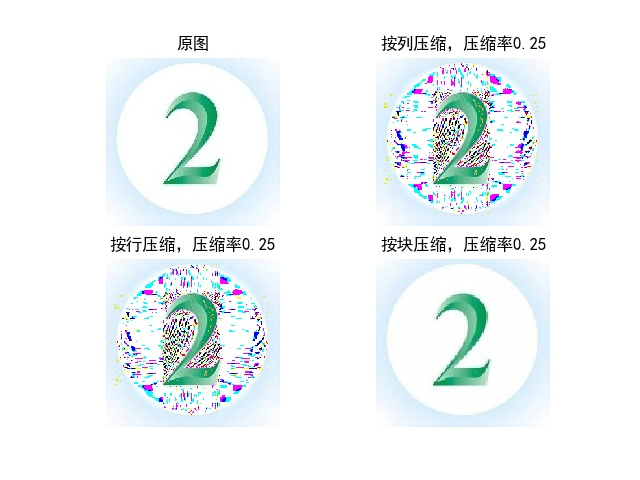
\includegraphics[width=.8\textwidth]{RGB.jpeg}
	\caption{RGB彩图PCA}
\end{figure}
\end{document}
